\documentclass[border=10pt,tikz]{standalone}
\usepackage{tikz}
\usetikzlibrary{positioning,arrows.meta,shapes}
\begin{document}
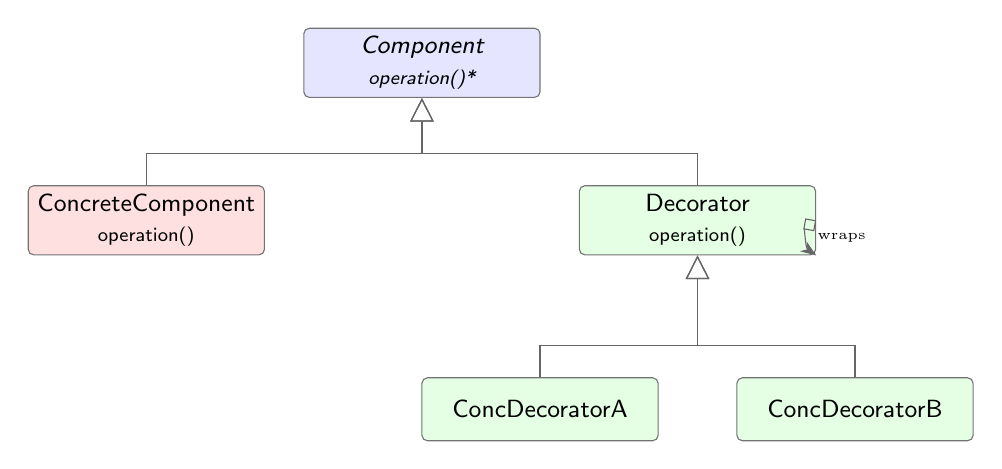
\begin{tikzpicture}[
  font=\sffamily\small,
  cls/.style={rectangle, rounded corners=2pt, draw=black!55, line width=0.4pt,
              minimum height=8mm, minimum width=30mm, inner sep=3pt, fill=white, align=center},
  abs/.style={cls, fill=blue!10, font=\sffamily\itshape\small},
  con/.style={cls, fill=red!12},
  imp/.style={cls, fill=green!10},
  inh/.style={-{Triangle[length=3mm,width=3mm,open]}, draw=black!60, line width=0.45pt},
  agg/.style={{Diamond[length=2mm,width=2mm,open]}-{Stealth[length=2mm]}, draw=black!60}
]
\node[abs] (com) at (0, 2)   {Component \\ \scriptsize operation()*};
\node[con] (cc)  at (-3.5,0) {ConcreteComponent \\ \scriptsize operation()};
\node[imp] (dec) at (3.5, 0) {Decorator \\ \scriptsize operation()};
\node[imp] (da)  at (1.5,-2.4) {ConcDecoratorA};
\node[imp] (db)  at (5.5,-2.4) {ConcDecoratorB};

\draw[inh] (cc.north) -- ++(0,0.4) -| (com.south);
\draw[inh] (dec.north) -- ++(0,0.4) -| (com.south);
\draw[agg] (dec.east) to[bend right=55] node[right, font=\tiny]{wraps} (dec.south east);
\draw[inh] (da.north) -- ++(0,0.4) -| (dec.south);
\draw[inh] (db.north) -- ++(0,0.4) -| (dec.south);
\end{tikzpicture}
\end{document}
